\documentclass{article}
\usepackage[utf8]{inputenc}
\usepackage{graphicx}

\title{PoC Implementation}
\author{Sophie Avard }
\date{October 2019}

\begin{document}

\maketitle

\section{Introduction}
Over the course of the semester my Proof of Concept has changed dramatically. As I have developed new digital skills and learnt new ways to analyse data, my Proof of Concept is now an R script that can convert pdf-to-txt, copy the files into a directory and import the data into a Shiny App which allows the data to be manually code. Additionally, I have written a script that cleans the csv file of the coded data. However, due to a bug in the Shiny app this could not be automated into my workflow so I have included it at the end with an example of coded data. While not all of my user stories have been met, this tool offers significant development potential. As such, my R script will:
\begin{enumerate}
    \item Convert pdf's into txt files
    \item Copy text files into Qcoder analysis directory 
    \item Import text files into Qcoder 
    \item Clean data that has been coded in Qcoder
\end{enumerate}

\section{User Stories}
Below is a breakdown of each user story explaining how it was met or why it was not met. A complete installation guide and instructions are provided in the User Manual. 

\subsection{Data Storage}
\begin{center}\textit{As a student, I want to store multiple sources of data in a single location so that the metadata and reference can be located efficiently.}
\end{center}
While I was able to successfully store data in Zotero and retrieve the metadata, this tool will not be used in my PoC. I feel as though storing my data in an organised directory is sufficient for the completion of this PoC. 

\subsection{Data Organisation}
\begin{center}\textit{As a student, I want all of my data named with the same format (consistent and descriptive) so that it is obvious where to find specific data and what the files contain.}
\end{center}

\subsection{Text Search}
As a student, I want my data analysis tool to have a search feature so that I can easily find phrases and words across multiple sources of data.
\begin{enumerate}
\item Open RStudio 
\item Run R script 
\item Select the relevant document 
\item Click on 'code data' 
\item Press Cmd + F
\item Search for word 
\end{enumerate}
Unfortunately, you cannot search for words across more than one source. However, there is potential for this later down the track.

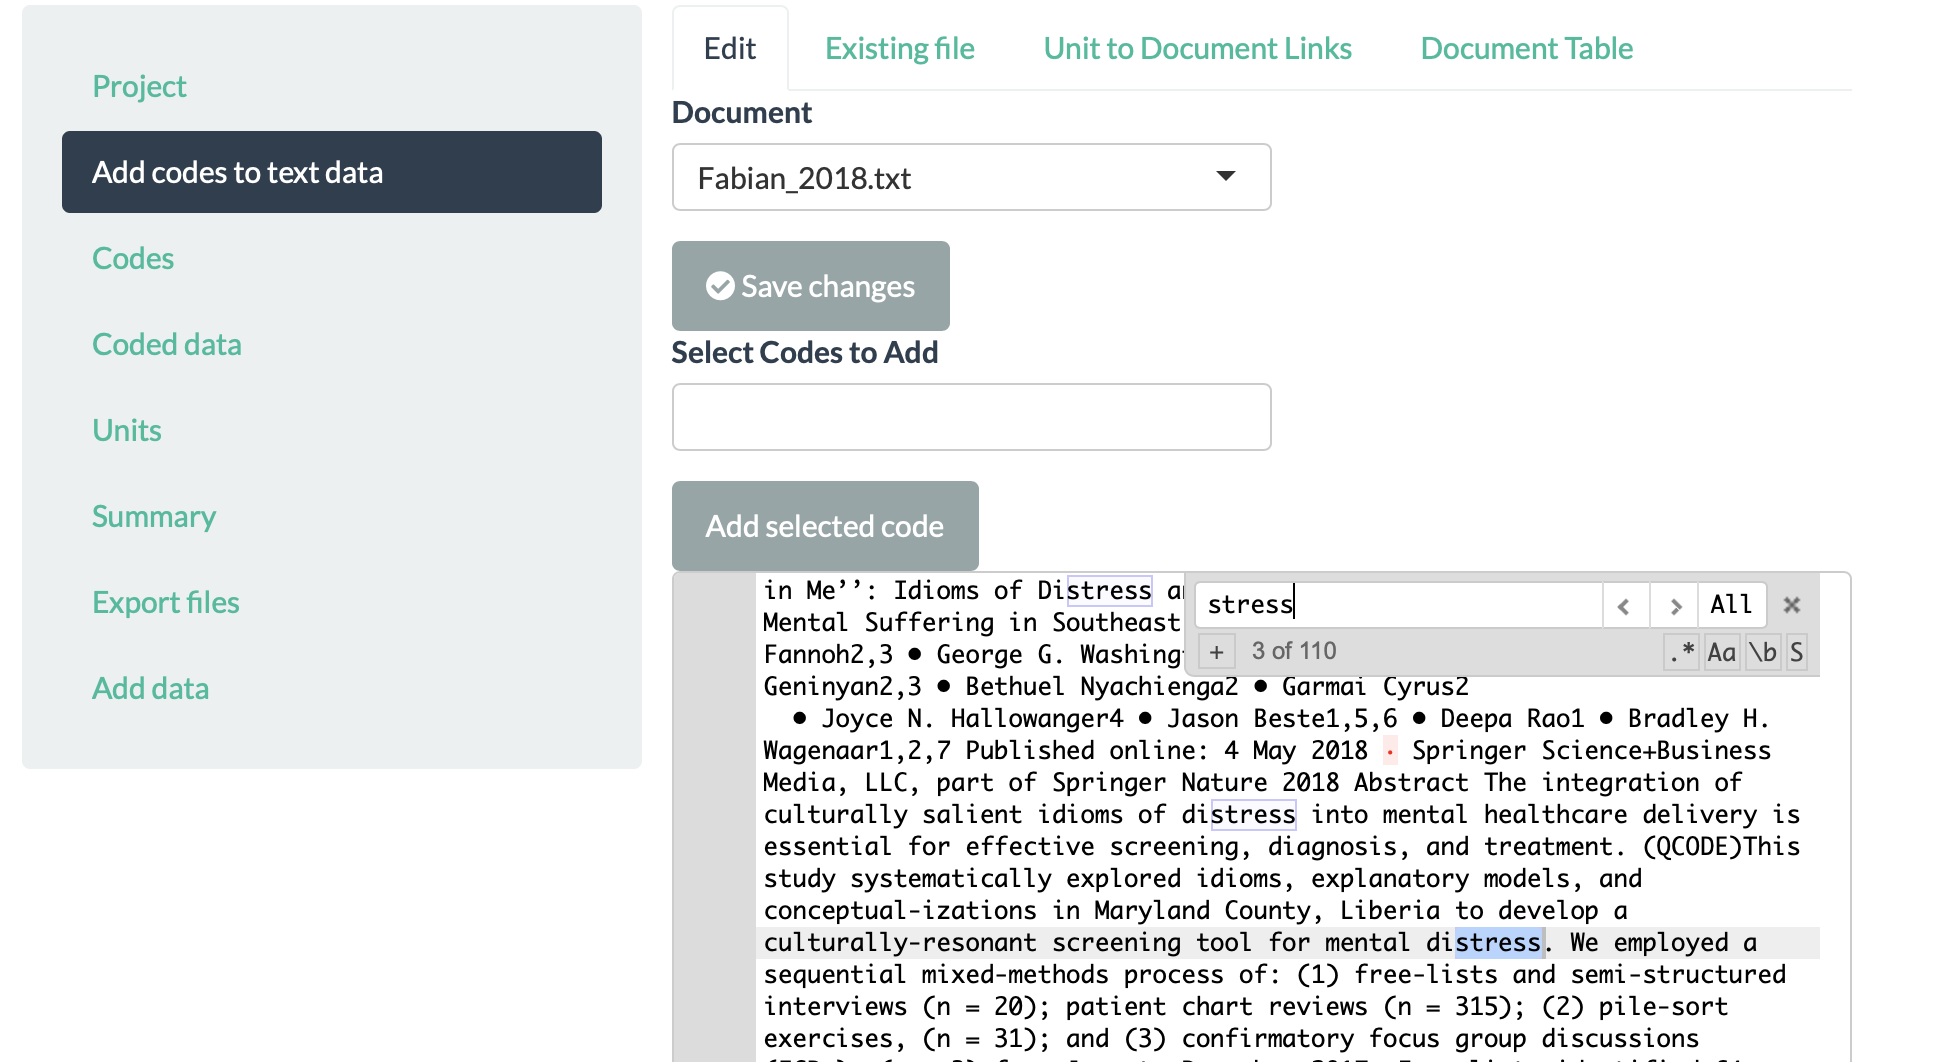
\includegraphics[width=\textwidth]{text-search.png}

\subsection{Tag Data}
As a student, I want my data analysis tool to create tags and add tags to sources so that I can identify patterns.
\begin{enumerate}
\item Run R script
\item Click select folder 
\item Click the relevant project 
\item Click 'add codes to text'
\item Select text to be coded
\item Add relevant code
\item Save Changes 
\item On the left click coded data
\end{enumerate}

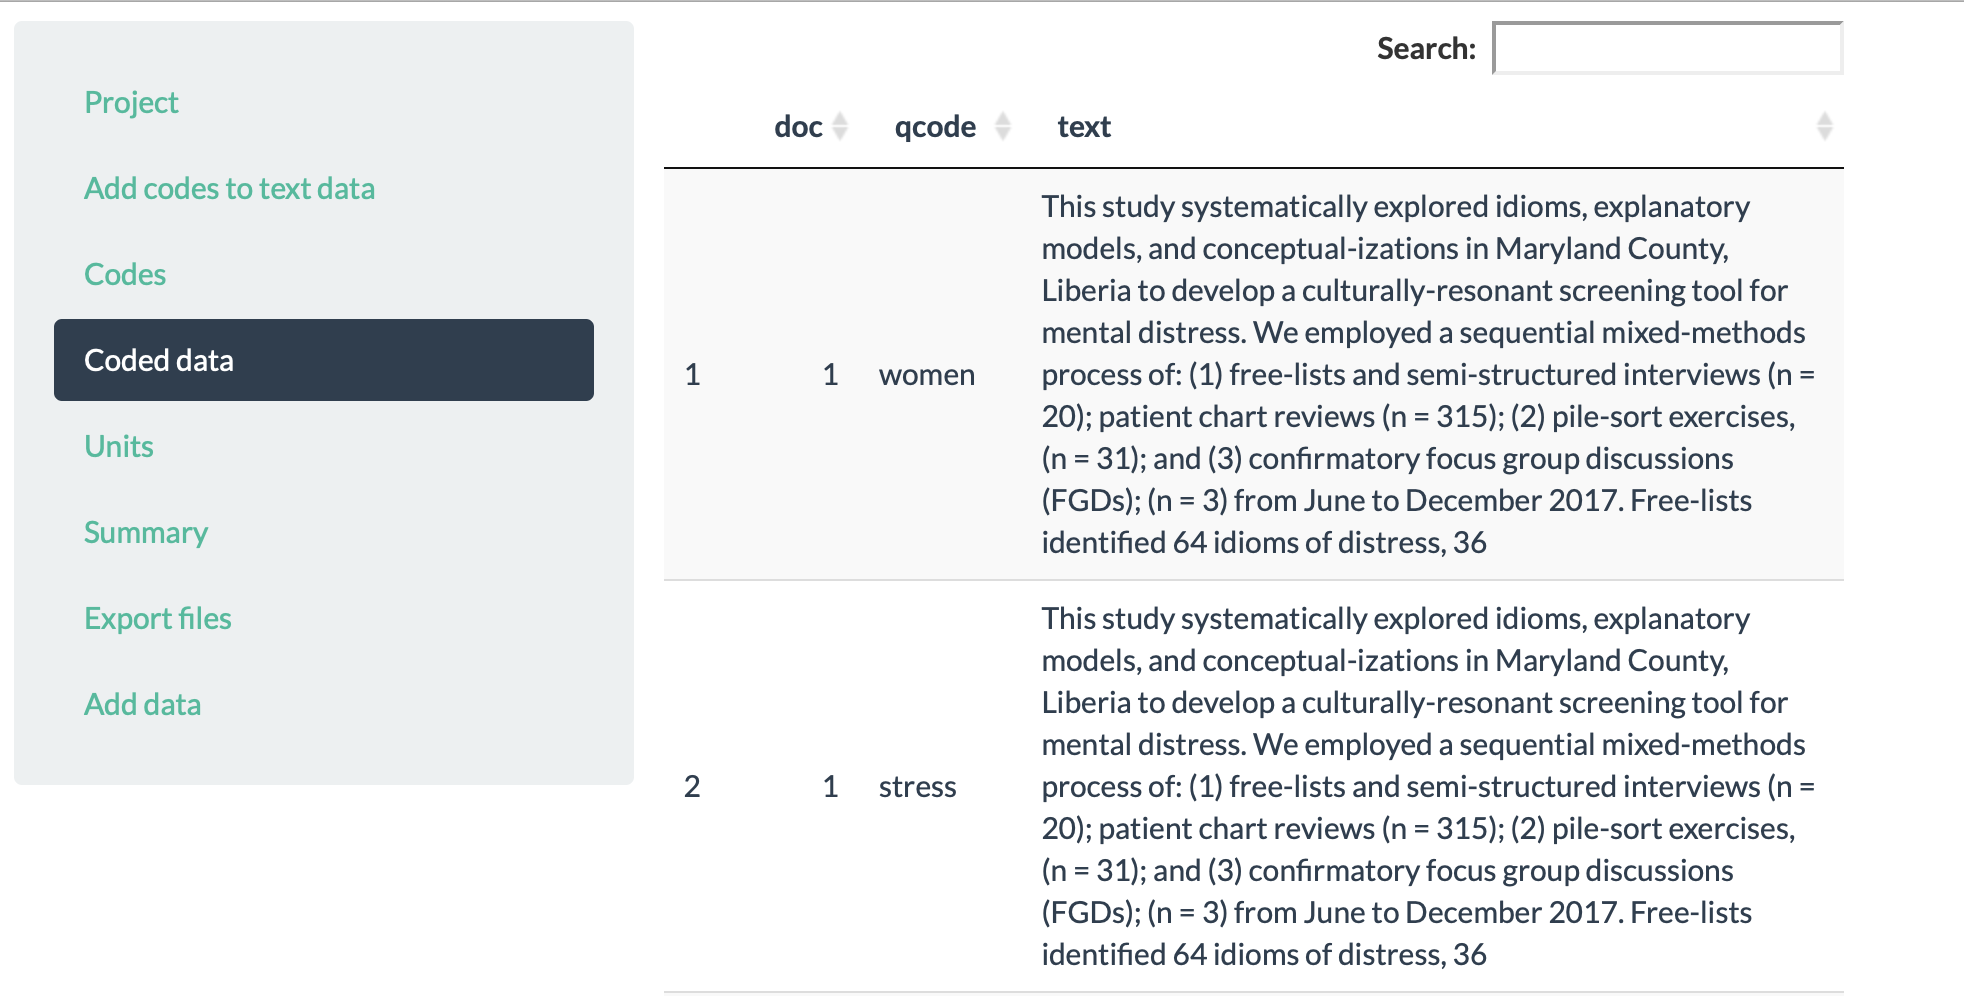
\includegraphics[width=\textwidth]{coded-data.png}


\subsection{Highlight Text}
As a student, I want my data analysis tool to allow me to highlight text to help me organise themes and connections between sources.
\begin{enumerate}
\item Run R script
\item Click select folder 
\item Click the relevant project 
\item Click 'add codes to text'
\item Select text to be coded
\item Add relevant code
\item Save Changes 
\item On the left click 'project'
\item Click 'existing file'
\item Document will be highlighted (see example below)
\end{enumerate}


\includegraphics[width=\textwidth]{highlight-text.png}


\subsection{Export Data Analysis}
As a student, I want my data analysis tool to export the tagged data in a csv format so that I can store it on my computer for later analysis. 
\begin{enumerate}
    \item Code the data following the instructiona above
    \item Click 'Coded data' on the left panel 
    \item Choose the export format (csv)
    \item Save with appropriate name 
\end{enumerate}
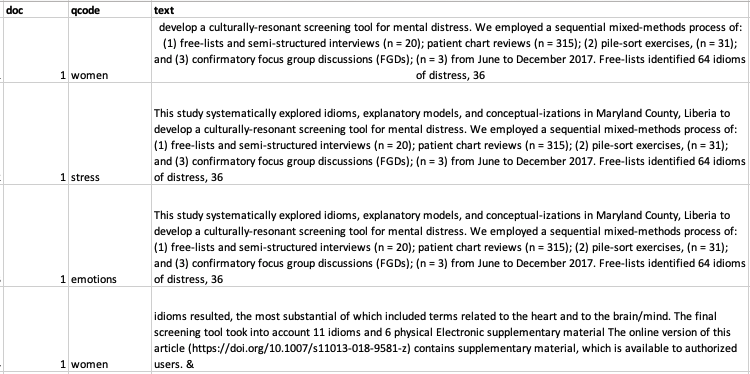
\includegraphics[width=\textwidth]{data-analysis-csv.png}

\end{document}
